\chapter{Play the Game}

Now that we have a board with the pieces on it, we actually want to play the game.

To that goal, we will explore how to make moves and store them for later usage.
Finally, we will consider special moves and positions to improve the game play.

\section{Making Moves}\label{sec:makemoves}

The first thing, we need for making moves, is a way to process user input.
We'll do that inside the event loop of the main fuction:

\begin{cpp*}{linenos}
// mouse button pressed
if (event.type == sf::Event::MouseButtonPressed) {
  if (event.mouseButton.button == sf::Mouse::Left) {
    pair<int, int> f = getField(event.mouseButton.x,
                                event.mouseButton.y);
    if (touched.first == -1) touched = f;
    else if (f == touched) touched = {-1, -1};
  }
}
// mouse button released
if (event.type == sf::Event::MouseButtonReleased) {
  if (event.mouseButton.button == sf::Mouse::Left) {
    pair<int, int> f = getField(event.mouseButton.x,
                                event.mouseButton.y);
    if (touched.first != -1 && touched != f)
      makeMove(board, moves, captured, touched, f, player);
  }
}

// get board coordinates
pair<int, int> getField(int x, int y) {
  int fx = x / 80;
  int fy = y / 80;
  auto field = make_pair(fy, fx);
  return field;
}
\end{cpp*}

We're using the \emph{left} mouse button for making moves (3, 12); remember that we've
used the right button for showing valid moves.\\
First, we need the coordinates of the board, where the mouse button was pressed (4),
respectively released (13).

When \emph{pressing} the button, and no field was touched yet (6), we set the variable\\
\mintinline{cpp}{pair<int,int> touched} to those coordinates.\\
But if a field was already touched, and it's the current field, we reset
\texttt{touched} (7).

When \emph{releasing} the button, we check wether a field was touched (15), and if it's not
the current field, we make a move from the touched to the current field (16).

With this mechanism, we can make a move in two ways:
\begin{itemize}
  \item \emph{drag-and-drop}: just move a piece from its current position to the target,
    while holding the left mouse button;
  \item \emph{click twice}: click once on the piece to move, and a second time on the
    target field.
\end{itemize}

The \mintinline{cpp}{getField()} function (21-26) converts the coordinates of the mouse cursor to
the coordinates of the board matrix.
Observe that it returns the coordinates in that order: first the row index, second the
column index.

In order to clean up the design, I decided to do some refactorings: I moved all function definitions,
except the main function, to a speparate implementation file
\texttt{app/moves.cpp}; and I moved all variable definitions into the main function, to get rid of
global variables.
So, we'll have the following definitions inside the main fuction:

\begin{cpp*}{linenos}
// matrix of pieces representing the board
vector<vector<Piece*>> board(8, vector<Piece*>(8));

// matrix of valid moves for display
vector<vector<short>> validMoves(8, vector<short>(8, 0));

// list of moves, used as a stack
auto* moves = new list::List<string>;

// list of captured pieces, used as a stack
auto* captured = new list::List<Piece*>;

// touched field for making moves
pair<int, int> touched{-1, -1};

// player to turn, starting with white
bool player = true;
\end{cpp*}

The variables \texttt{moves} and \texttt{captures} are \emph{linked lists}, which I've implemented
in a separate library called \texttt{datastructures} within a namespace \texttt{list}.
I will not go into details here, but if you are interested in implementing a linked list for yourself,
have a look at the file \texttt{include/list.hpp} in that directory (it's quite well documented,
so you should find your way around).

But now, to the most important function of this section: \mintinline{cpp}{makeMove()}.

\begin{cpp*}{linenos}
void makeMove(vector<vector<Piece*>>& bd,
              list::List<string>* mv,
              list::List<Piece*>* cp,
              pair<int, int>& td,
              pair<int, int> to,
              bool& player)
{
  auto pcf = bd[td.first][td.second];
  auto pct = bd[to.first][to.second];
  bool cap = false;
  if (!pcf) {
    cout << "no piece under cursor\n";
    td = {-1, -1};
    return;
  }
  if (pcf->isWhite() != player) {
    cout << "it's not your turn\n";
    td = {-1, -1};
    return;
  }
  if (pcf->isValid(bd, to.first, to.second)) {
    if (pct && pct->isWhite() != pcf->isWhite()) {
      cap = true;
      pct->capture();
      cp->push_front(pct);
    } else if (pct) {
      cout << "illegal move!\n";
      td = {-1, -1};
      return;
    }
    mv->push_front(convertFromBoard(cap, pcf, to));
    bd[to.first][to.second] = pcf;
    bd[td.first][td.second] = nullptr;
    pcf->makeMove(to.first, to.second);
    td = {-1, -1};
    player = !player;
    cout << mv->peek(1) << "\n";
  // illegal move
  } else {
    cout << "illegal move!\n";
    td = {-1, -1};
  }
}
\end{cpp*}

First, we get the pieces of the start (\texttt{td}, the touched field) and target coordinates (\texttt{to})
of the move(8, 9).\\
If there's no piece at the start coordinates (11), reset the touched field (13) and abort the move (14).\\
If the color of the start piece doesn't match the player, whose turn it is (16), also abort the move (19).

Otherwise, check wether the move is valid (21), and wether the piece at the target position can be
captured (22).\\
If so, capture the piece (24) and and push it onto the stack of captured pieces (25).\\
Otherwise, if there's a piece of the same color (26), abort the move (29).

So far, we've checked all the possible variations and have a valid move; thus, we add the move to the
stack of moves (31).\\
Then, we set the piece under the cursor to its target position on the board (32), overwriting the old
reference, and delete its old postion (33).

Finally, we tell the piece its new position (34), reset the touched field (35), and switch to the other

For pushing the move onto the moves stack, I used a function \mintinline{cpp}{convertFromBoard} (31),
which is defined like so:

\begin{cpp}
string convertFromBoard(bool cap, Piece* from, pair<int, int> to) {
  string move;
  char type = from->getType();
  if (type != 'P') {
    move.append(1, type);
  }
  move.append(1, colToFile(from->getCol()));
  move.append(1, rowToRank(from->getRow()));
  if (cap) {
    move.append(1, 'x');
  } else {
    move.append(1, '-');
  }
  move.append(1, colToFile(to.second));
  move.append(1, rowToRank(to.first));
  return move;
}

char colToFile(int col) {
  char file = 97 + col;
  return file;
}

char rowToRank(int row) {
  char rank = 56 - row;
  return rank;
}
\end{cpp}

The function takes a piece (\texttt{from}) and target coordinates (\texttt{to}) as parameters,
and converts them into a string of
\href{https://en.wikipedia.org/wiki/Algebraic_notation_(chess)}{algebraic chess notation}.\\
It makes use of two helper functions \mintinline{cpp}{colToFile()} and \mintinline{cpp}{rowToRank()},
which convert the coordinates of the board matrix to chess coordinates.

Those functions use a little trick, based on the specification of the \mintinline{cpp}{char} type in
C\textsuperscript{++}: the actual value of a character is stored as a \mintinline{cpp}{short int},
based on the ascii code for that character.
So, the letter `a' is stored internally as 97, and the digit `8' as 56. We use this fact for a
simple calculation.

The only thing left to do is to adjust the \mintinline{cpp}{resetBoard()} function to take care of
the moves stack and the captured pieces:

\begin{cpp}
void resetBoard(vector<vector<Piece*>>& bd,
                 list::List<string>* mv,
                 list::List<Piece*>* cp)
{
  // reset moves and captured pieces
  delete mv;
  mv = new list::List<string>;
  delete cp;
  cp = new list::List<Piece*>;
  // reset board
  for (auto rank : bd) {
    for (auto piece : rank) {
      delete piece;
    }
  }
  // --- snip ---
}
\end{cpp}

We have to explicitly delete the moves stack and the stack of captured pieces when resetting to board,
in order to avoid memory leaks.
But then, we have to create them again as empty lists, as we want to use them for the next game.
Notice, that not only the references to those lists are deleted, but also all elements inside the lists,
due to that destructor in the file \texttt{datastructures/include/list.hpp}:

\begin{cpp}
template<typename T>
class List : public LL<T> {
public:
  ~List() {
    Node* node = head;
    while(node) {
      Node* curr = node;
      node = node->next;
      delete curr;
    }
    delete node;
  }
}
\end{cpp}

The very last thing, we want to do in this section, is to add a marker inside the main function for the
touched piece on the board

\begin{cpp}
sf::RectangleShape frame(sf::Vector2f(63.f, 60.f));
frame.setFillColor(sf::Color(200, 200, 200, 50));
frame.setOutlineThickness(12.f);
frame.setOutlineColor(sf::Color(100, 100, 0));
\end{cpp}

and draw it together with the pieces inside the game loop:

\begin{cpp}
// draw pieces
for (int row = 0; row < 8; row++) {
  for (int col = 0; col < 8; col++) {
    if (board[row][col]) {
      auto piece = board[row][col];
      // --- snip ---
      if (row == touched.first && col == touched.second) {
        frame.setPosition(col*80.f + 10.f, row*80.f + 10.f);
        window.draw(frame);
      }
      pc.setPosition(col*80.f + 10.f, row*80.f + 10.f);
      window.draw(pc);
    }
  }
}
\end{cpp}

\section{Special Positions}\label{sec:specpos}

The most prominent position in a game is the \href{https://en.wikipedia.org/wiki/Check_(chess)}{check},
where the king is under immediate attack.
So far, we have no mechanism to respond to or even detect a \emph{check}.
Let's change that now.

For that, we only need to iterate over all opponent pieces, and if any of them can reach the king
with a valid move, we have a check:

\begin{cpp*}{linenos}
bool check(vector<vector<Piece*>>& bd, bool white) {
  Piece* king;
  bool check = false;
  for (int row = 0; row < 8; row++) {
    for (int col = 0; col < 8; col++) {
      auto current = bd[row][col];
      if (current && current->getType() == 'K' &&
          current->isWhite() == white)
      {
        king = current;
      }
    }
  }
  for (int row = 0; row < 8; row++) {
    for (int col = 0; col < 8; col++) {
      auto current = bd[row][col];
      if (current && current->isWhite() != white) {
        if (current->isValid(bd, king->getRow(), king->getCol())) {
          check = true;
        }
      }
    }
  }
  return check;
}
\end{cpp*}

First, iterate over all positions of the board (4-5) and check wether the piece at that position
is the king of the given color (7-8).
If so, store the position of the king (10).

Then, iterate again over all positions of the board (14-15) and check wether there's a piece
of the opponent color (17).
If so, check wether this piece can reach the king with a valid move (18), and if it can,
set the position to \emph{check} (19).

With that, we have two searches with 64 tests each, and we need to run them sequentially,
resulting in 128 tests.
Now you could think that's superfluous, as we could test only against the piece actually beeing
moved, reducing the second search to a single test.
But you would be wrong: a check can be given by any other piece, if a blocking piece is moved.
Convince yourself with this diagram:

\begin{center}
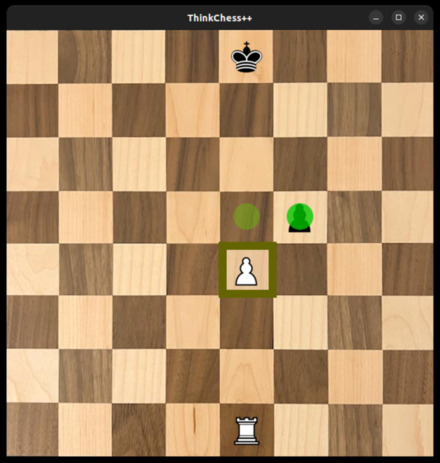
\includegraphics[width=.5\linewidth]{img/check.jpg}
\end{center}

If white captures the black pawn on \texttt{f5} with \texttt{e4xf5+}, the white rook on the
\texttt{e}-file will give the black king check.

Now, before making the move, let's look at the other special (and terminal) position: \emph{checkmate}.
If a player, given check in the last move, cannot respond to the check in the very next move, that
players king is checkmate, and the game is over.

There are, in general, three ways to get out of check:

\begin{enumerate}
  \item capturing the checking piece
  \item moving the king
  \item blocking the check.
\end{enumerate}

It's the players duty to analyze the position and to find the best solution.
For now, our app cannot do this, it'a a quite complex task.\\
But thankfully, it doesn't have to: we only want to detect a checkmate and decide wether the game
is over at this point.\\
For that, we dont't need any fancy alorithm or some kind of intelligence, we just use a
\href{https://en.wikipedia.org/wiki/Brute-force_search}{brute-force} search.
Instead of finding the best solution, we only need to know if there is \emph{any} solution:

\begin{cpp*}{linenos}
bool resolveCheck(vector<vector<Piece*>>& bd, bool white) {
  for (int row = 0; row < 8; row++) {
    for (int col = 0; col < 8; col++) {
      auto current = bd[row][col];
      // get every piece of given color
      if (current && current->isWhite() == white) {
        for (int rr = 0; rr < 8; rr++) {
          for (int cc = 0; cc < 8; cc++) {
            if (current->isValid(bd, rr, cc)) {
              auto pct = bd[rr][cc];
              if (!pct || pct->isWhite() != white) {
                // make move and test for check
                bd[rr][cc] = current;
                current->makeMove(rr, cc);
                if (!check(bd, white)) {
                  bd[rr][cc] = pct;
                  current->makeMove(row, col);
                  return true;
                } else {
                  bd[rr][cc] = pct;
                  current->makeMove(row, col);
                }
              }
            }
          }
        }
      }
    }
  }
  return false;
}
\end{cpp*}

Iterate over all fields of the board (2-3); if there's a piece at this postion with the color of the
checked player (6), start another nested loop (7-8) to get the valid moves of that piece (9).\\
If the reachable fields are empty or the pieces at these positions are of the other color
(i.e. they can be captured), make this move by setting the current piece to this position (13-14).

If this new position is not giving check (15), we have a solution and return \mintinline{cpp}{true},
indicating that the check could be resolved with that move (18).\\
But, before doing so, reset the board to its original state, as we don't want to actually make
the move (16-17).

If the new position still is giving check (19), reset the board as well (20-21) and continue the search.

With that, we have four nested loops with $8 \times 8 \times 8 \times 8 = 64 \times 64 = 4096$ tests,
which isn't optimal; but that's the cost of \emph{brute search}.

On the other  hand, any decent CPU can handle about \emph{one billion} of those simple tests per
second.
So, calling that function will take less than a microsecond on average, for which we have
surely enough time (remember, the framrate is set to 10, so we have
100 microseconds for every frame).

With all that in place, we can finally make a move, while testing for \emph{check} and \emph{checkmate}:

\begin{cpp*}{linenos}
void makeMove(vector<vector<Piece*>>& bd,
              list::List<string>* mv,
              list::List<Piece*>* cp,
              pair<int, int>& td,
              pair<int, int> to,
              bool& player,
              pair<int, int>& checkmate)
{
  auto pcf = bd[td.first][td.second];
  auto pct = bd[to.first][to.second];
  bool cap = false;
  if (!pcf) {
    cout << "no piece under cursor\n";
    td = {-1, -1};
    return;
  }
  if (pcf->isWhite() != player) {
    cout << "it's not your turn\n";
    td = {-1, -1};
    return;
  }
  // valid move?
  if (pcf->isValid(bd, to.first, to.second)) {
    // can capture?
    if (pct && pct->isWhite() != pcf->isWhite()) {
      cap = true;
      cp->push_front(pct);
    } else if (pct) { // same color
      cout << "illegal move!\n";
      td = {-1, -1};
      return;
    }
    // legal move
    string move = convertFromBoard(cap, pcf, to);
    bd[to.first][to.second] = pcf;
    bd[td.first][td.second] = nullptr;
    pcf->makeMove(to.first, to.second);
    // check?
    if (check(bd, player)) { // gives itself check
      cout << "illegal move!\n";
      bd[to.first][to.second] = pct;
      bd[td.first][td.second] = pcf;
      pcf->makeMove(td.first, td.second);
      td = {-1, -1};
      return;
    }
    if (check(bd, !player)) { // gives opponent check
      if (resolveCheck(bd, !player)) {
        move.append(1, '+');
      } else { // cannot get out of check
        move.append(1, '#');
        mv->push_front(move);
        cout << mv->peek(1) << "\n";
        checkmate = getKing(bd, !player);
        return;
      }
    }
    mv->push_front(move);
    cout << mv->peek(1) << "\n";
    td = {-1, -1};
    player = !player;
  // illegal move
  } else {
    cout << "illegal move!\n";
    td = {-1, -1};
  }
}
\end{cpp*}

There's nothing new in lines (1-37).
Then test, wether the move gives the own king check (39), and if it does, abort the move (44-45), as
this is not allowed.\\
But, before that, reset the already made move (41-43).

If the move gives the opponents king check (47), test wether the check could possibly be
resolved (48), and if so, add the marker `+' to the move (indicating check, 49).\\
If the check cannot be resolved (50), add the marker `\#' to the move (indicating checkmate, 51),
push the move to the moves stack (52), and set the \texttt{checkmate} variable to the postion
of the checkmated king (54).\\
Then, proceed as before (58-67).

We use the \texttt{checkmate} variable to to stop the game and draw a corresponding marker on the board
within the main function of the app):

\begin{cpp}
short state = 1;
pair<int, int> checkmate{-1, -1};

//marker for checkmate
sf::RectangleShape cm(sf::Vector2f(63.f, 60.f));
cm.setFillColor(sf::Color(200, 200, 200, 50));
cm.setOutlineThickness(12.f);
cm.setOutlineColor(sf::Color(200, 0, 0));

// game loop
while (window.isOpen()) {
  // event loop
  for (auto event = sf::Event{}; window.pollEvent(event);) {
    if (event.type == sf::Event::Closed) {
      window.close();
    }
    // mouse button pressed
    if (event.type == sf::Event::MouseButtonPressed) {
    // --- snip ---
      if (event.mouseButton.button == sf::Mouse::Left) {
        if (state == 1) {
          pair<int, int> f =
            getField(event.mouseButton.x, event.mouseButton.y);
          if (touched.first == -1) touched = f;
          else if (f == touched) touched = {-1, -1};
        }
      }
    }
    // mouse button released
    // --- snip ---
      if (event.mouseButton.button == sf::Mouse::Left) {
        if (state == 1) {
          pair<int, int> f =
            getField(event.mouseButton.x, event.mouseButton.y);
          if (touched.first != -1 && touched != f)
            makeMove(board, moves, captured,
                     touched, f, player, checkmate);
        }
      }
    }
  } // end event loop

  // draw pieces
  for (int row = 0; row < 8; row++) {
    for (int col = 0; col < 8; col++) {
      if (board[row][col]) {
      // --- snip ---
        if (row == checkmate.first && col == checkmate.second) {
          cm.setPosition(col*80.f + 10.f, row*80.f + 10.f);
          window.draw(cm);
        }
        pc.setPosition(col*80.f + 10.f, row*80.f + 10.f);
        window.draw(pc);
      }
    }
  }
  // display frame
  window.display();

  // stop game when checkmate
  if (checkmate.first != -1) state = 0;
\end{cpp}

And here you have it: a fully playable chess app for two players!

Playing the moves
\begin{verbatim}
1. e2-e4 e7-e5
2. Ng1-f3 Ng8-f6
3. Nf3xe5 Nf6xe4
4. Qd1-f3 Ne4-c5
5. Qf3xf7#
\end{verbatim}

will lead to this position, correctly identified as checkmate, also known as a variant of
the \emph{Scholar's mate}:

\begin{center}
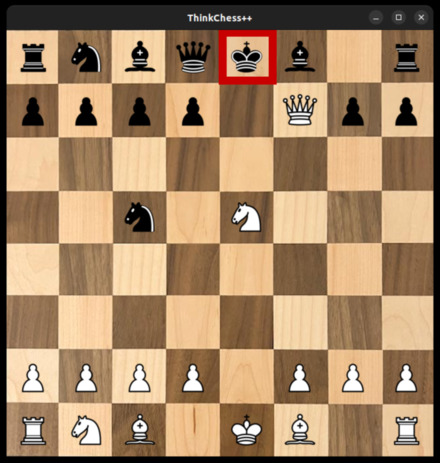
\includegraphics[width=.5\linewidth]{img/checkmate.jpg}
\end{center}


\section{Special Moves}\label{sec:specmoves}
